\chapter{FPGA Acceleration of CIPRNGs}
In this chapter, the proposition is to improve widely the efficient of the formerly proposed generators, without any lack of chaos properties. To do that, Field programmable gate array (FPGA) method is proposed.

\section{introduction}
Nowadays, FPGAs are very successfully applied to implement random sequence generation due to its ability in highly parallelizable task \cite{Bojani200663, Danger:2009:HST:1645457.1645933, Tsoi:2003:CFT:938383.938400}. Such device allows us to generate pseudorandom numbers with remarkable speed. In these and other implementations, FPGA has advantages in performance, design time, power consumption, flexibility, cost and so on.

According to the previous chapters' description, it has proven that the chaotic iterations (CIs), to be a very decent tool for computing iterative algorithms, satisfies the chaos property, as it is defined by Devaney. The chaotic behaviour of CIs is developed attempt to obtain an unpredictable PRNG, in \cite{DBLP:journals/corr/abs-1112-5239}, its efficient implementations on GPU have been designed in, expressing that a very large quantity of pseudorandom numbers can be generated per second. Here, generators based on chaotic iteration is designed specifically for FPGA hardware, with that, the rate of generation can be hugely increased.

\section{FPGA design}
\label{FPGA design}
In order to take benefits from the computing power of FPGA, a whole processing needs to spread into several independent blocks  of threads that can be computed simultaneously. In general,  the larger the number of  threads is, the more logistic elements of FPGA are used, and the less branching  instructions are used  (if,  while,  ...),  the  better the  performances  on  FPGA  is. Obviously, having these requirements in  mind, suitable CIPRNG algorithms which produce random numbers with chaotic properties should be chosen to apply to FPGA. The Verilog-HDL~\cite{verilog} is used to help program. 

\subsection{CI Version selection}
According to the comparison in Chapter~\ref{Statistical Tests for Randomness}, it can be seen that Version 4 CI algorithms is the most adaptable of all, its loop processing of them are both able to be replaced by parallel computing to increase the efficiency. To be noticed, the CIPRNGs used here are both proven to be cryptographically secure (check Section~\ref{Security Analysis}) by using BBS and three XORshift PRNGs, and its statistical performance is withstand the TestU01 test suite (Section~\ref{test for Version 4 CI}).
\subsection{Design of XORshift}
The structure of PRNG XORshift designed in Verilog-HDL is shown in Figure
\ref{xorshift verilog}, there are four inputs, first one is the initial state, which cost 64 bits 
of register units, then the other three ones are used to define how to shift, in FPGA, shifting cost no 
elements (just using different bit cell of the input). Then there are $64 - s1 + 64 -s2 + 64 -s3 
= 192 - s1 - s2 - s3$ logic gates elements applied for XORshift processing. In program, we define 
each FPGA clock positive edge, the XORshift will work, since these are simple processing for FPGA, every 
clock step can lead to one output.
\begin{figure}
\begin{center}
  \subfigure[XORshift]{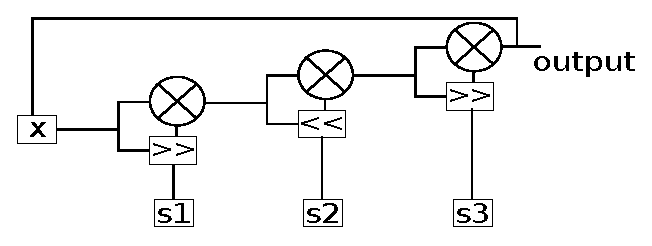
\includegraphics[width=6.5cm]{xorshift.eps}
  \label{xorshift verilog}}
  \subfigure[BBS]{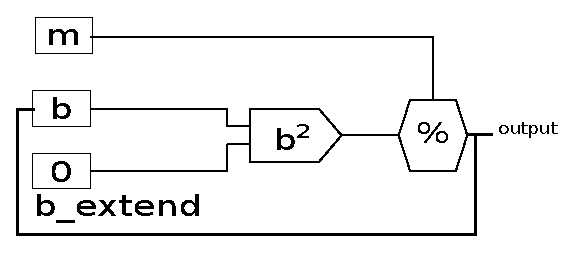
\includegraphics[width=6.5cm]{bbs.eps}
  \label{BBS verilog}}
\end{center}
\caption{The structure of processing for XORshift and BBS in FPGA each clock step}
\end{figure}

\subsection{Design of BBS}
Figure~\ref{BBS verilog} gives the design of BBS in FPGA, there are two $32$ bits length input: 
$b$ and $m$, $m$ is also a register stores the value of M which will not be changed, register $b$ 
stores the every time state, when it is processing square computation, another register $b\_extend$ 
is used to combine with $b$ to a $64$ bits length data to avoid overflow. At last output is taking 
the three LSBs from the output of $\%$ as output. BBS performs the function while every positive 
edge of clock.

\subsection{Design of the Version 4 CI}
For composition of the CI PRNG, two XORshifts and BBS are connected to work together (Figure~\ref{CI verilog}), 
as shown, the three bits of the output of BBS are the switches for the corresponding $32$ bits from 
XORshift outputs. Every round of the CI RPNG processing costs two times clock positive edge to finish: In first clock, 
the four PRNGs are processed in parallel; Then in second clock, the results of the classic PRNGs are combined with 
the state to produce the output ($32$ bits binary).


\begin{figure}
 \begin{center}
 
  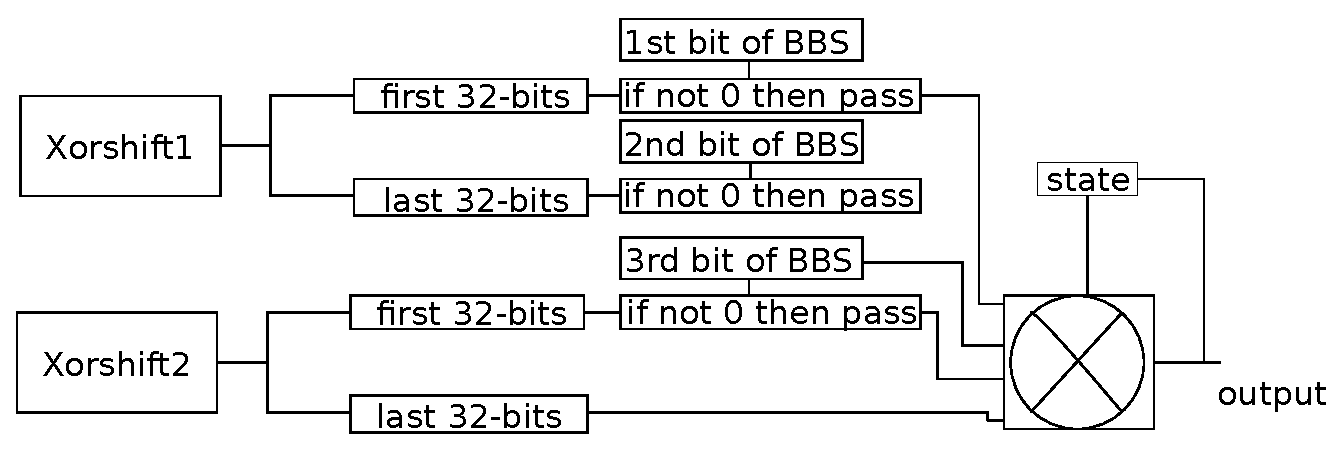
\includegraphics[width=10cm]{ci.eps}
  \label{CI verilog}
  \caption{The structure of CI PRNG in FPGA}
 \end{center}
\end{figure}

In our experiment, type $EP2C8Q208C8$ from Altera 
company's CYCLONE II FPGA series is applied, it can 
give $50$ MHz working clock frequency in default,
with the help of phase-lock loop (PLL) device, the frequency could be increased into 
$400$ MHz,then our generator based on CI can achieve $400 (MHz) \div 2 (times) \times 32 (bits)$
which can achieve about $6400$ Mbits per second, and there are 100 logic elements used totally, 
that only takes $1\%$ in $EP2C8Q208C8$ ($100$ from $8256$ logic elements shown in 
Figure~\ref{logic elements}). 
In next section, an information hiding 
application is expressed by the FPGA device.

\begin{figure}
\begin{center}
  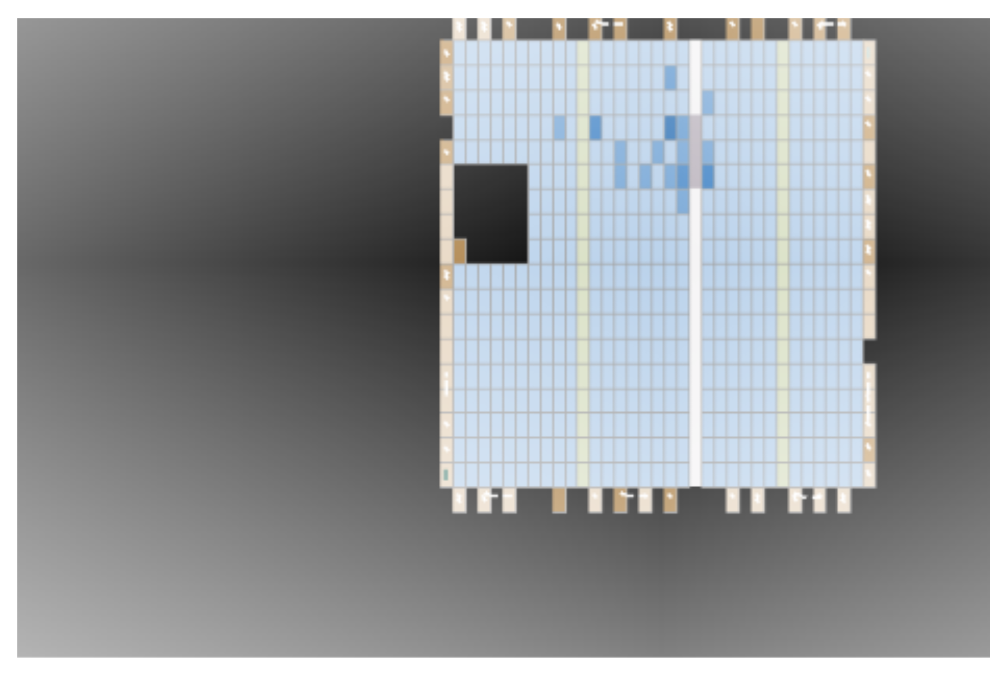
\includegraphics[width=6.5cm]{print.eps}
\end{center}
\caption{The sources cost in $EP2C8Q208C8$ FPGA board}
 \label{logic elements}
\end{figure}

